\renewcommand{\chaptername}{Chapter} 
\chapter{Perseveration analysis}\label{chap9}

\section{Perseveration analysis} 
\subsection{Trial difficulty} 

\subsection{Number of identical responses} 
\begin{figure}[H]
    \centering
    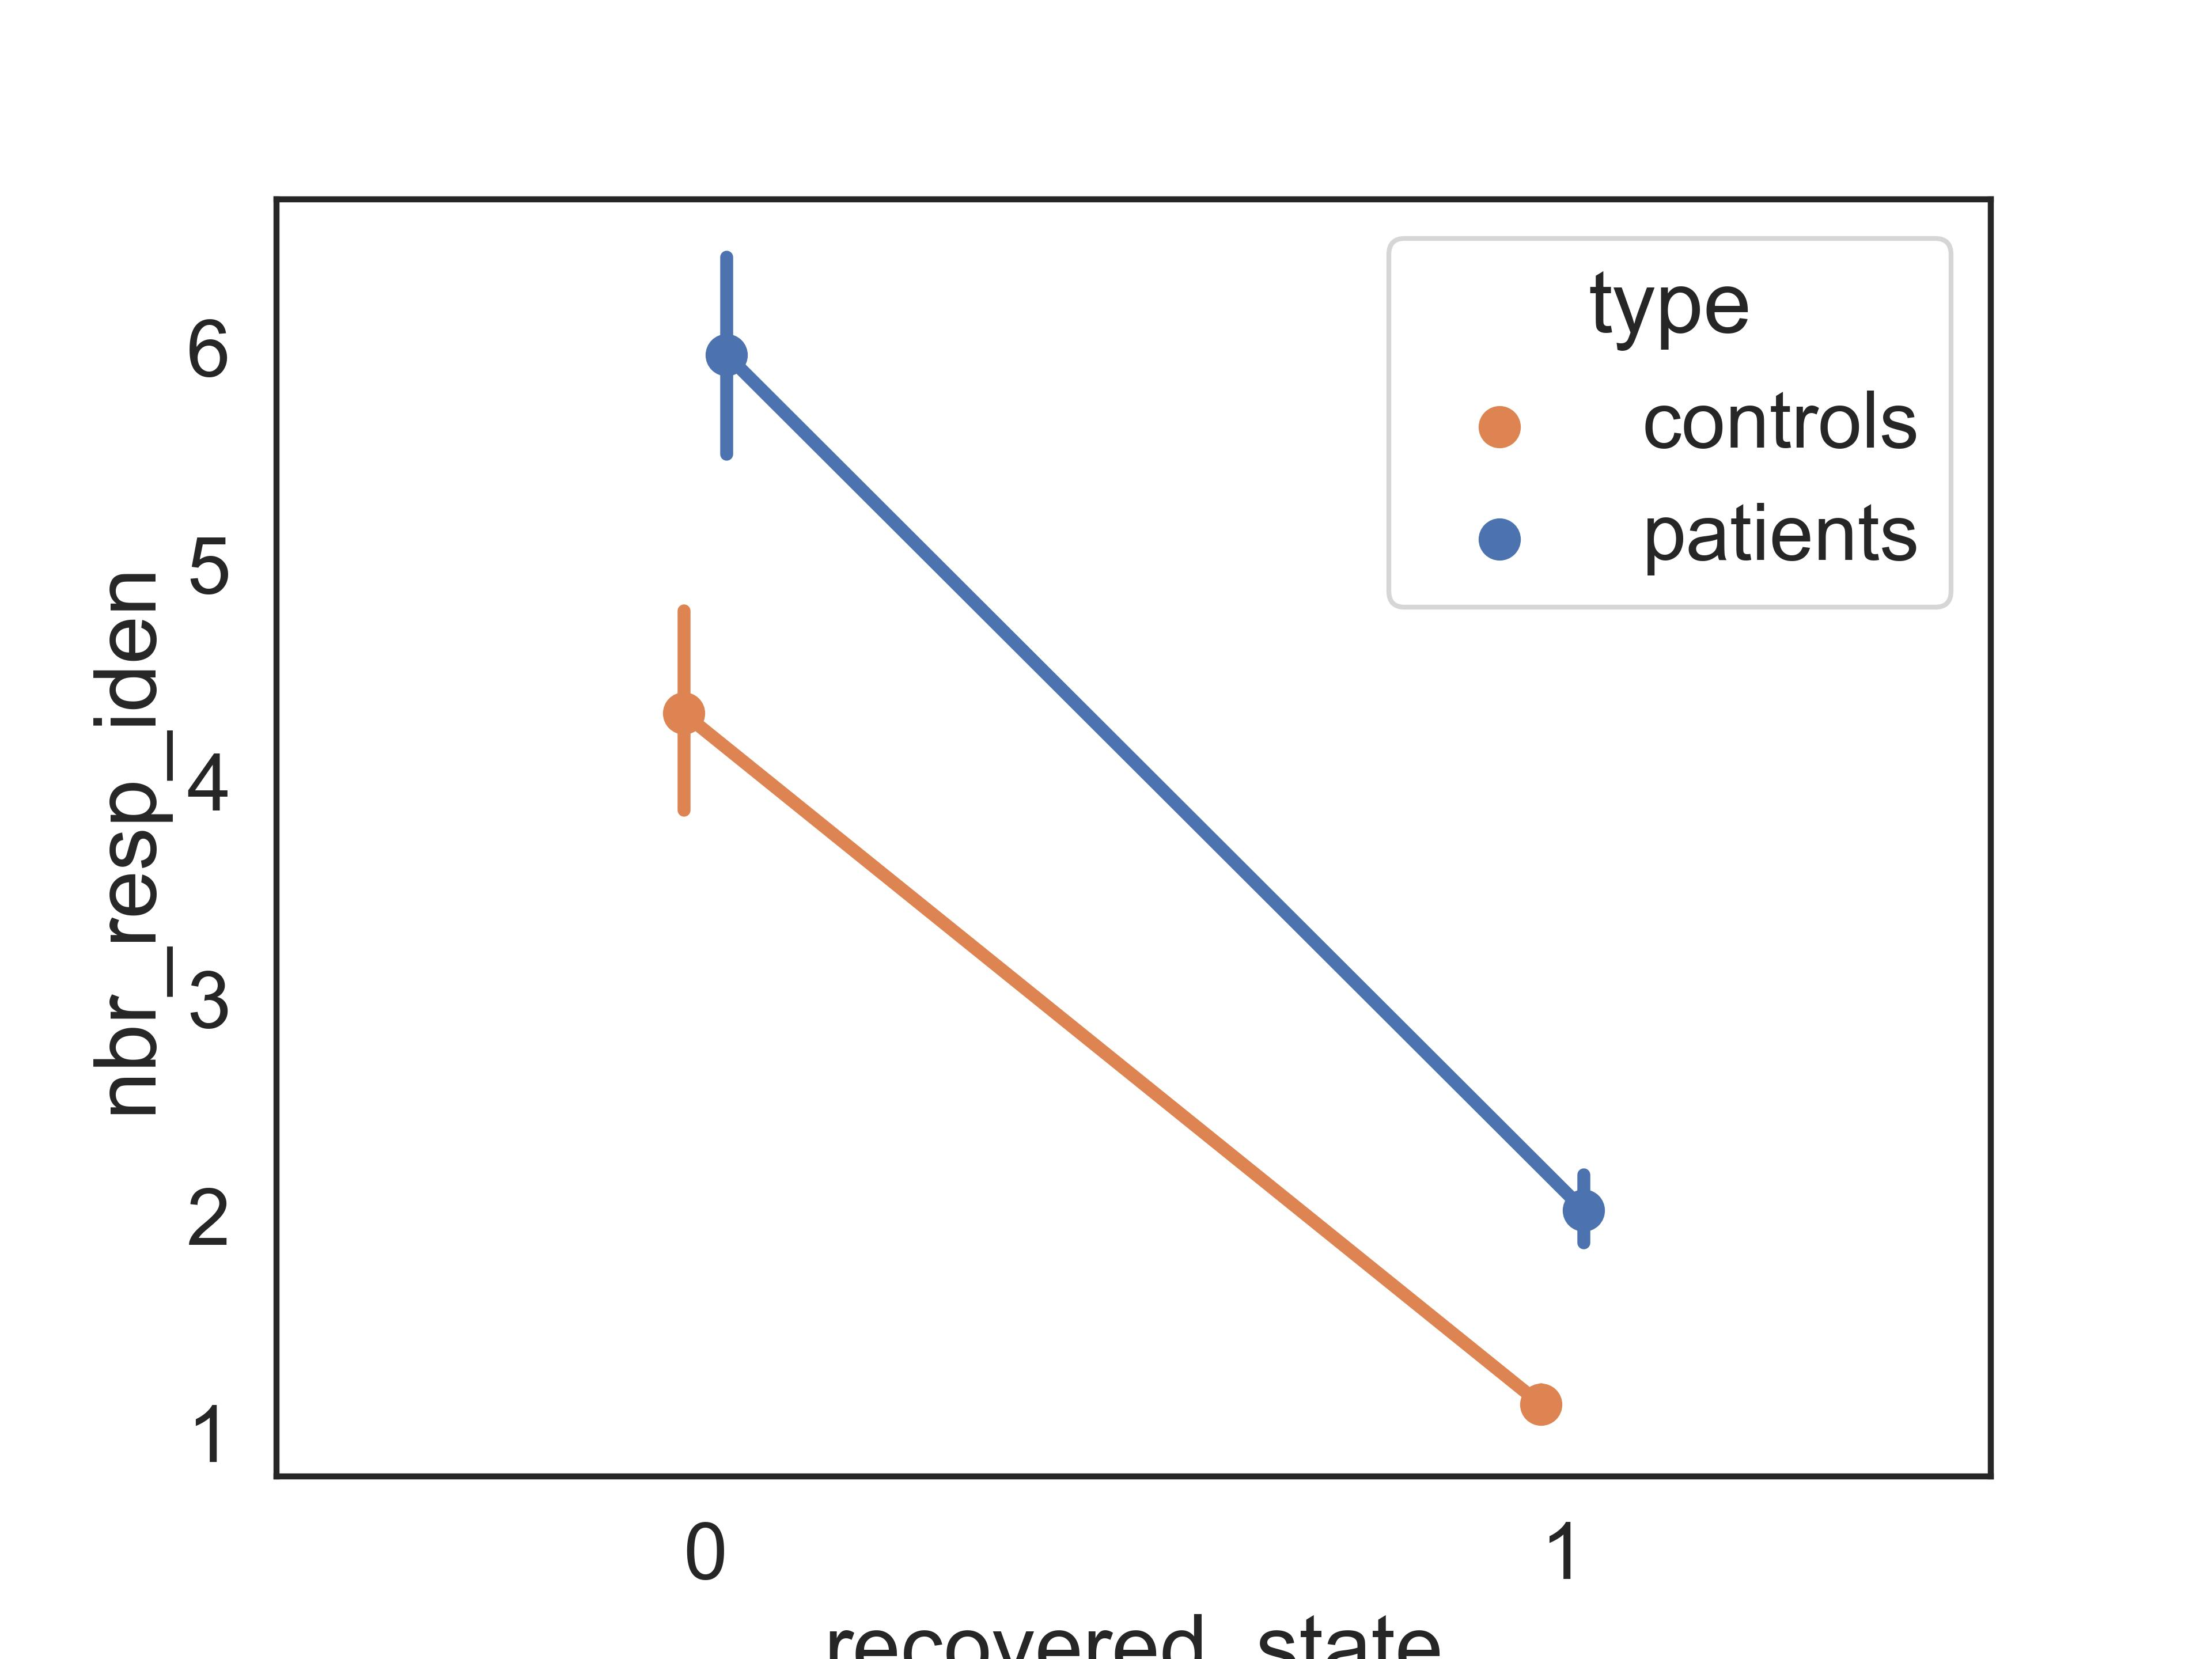
\includegraphics[width=12cm,height=7cm]{MainLayout/Images/chapter9/nbr_resp_iden.jpg}
    \caption{Main Title for First Image \\ \small Subtitle for the first graphic.}
    \label{fig:kernel_comparison_methods}
\end{figure}

\subsection{Expected responses} 
\begin{figure}[H]
    \centering
    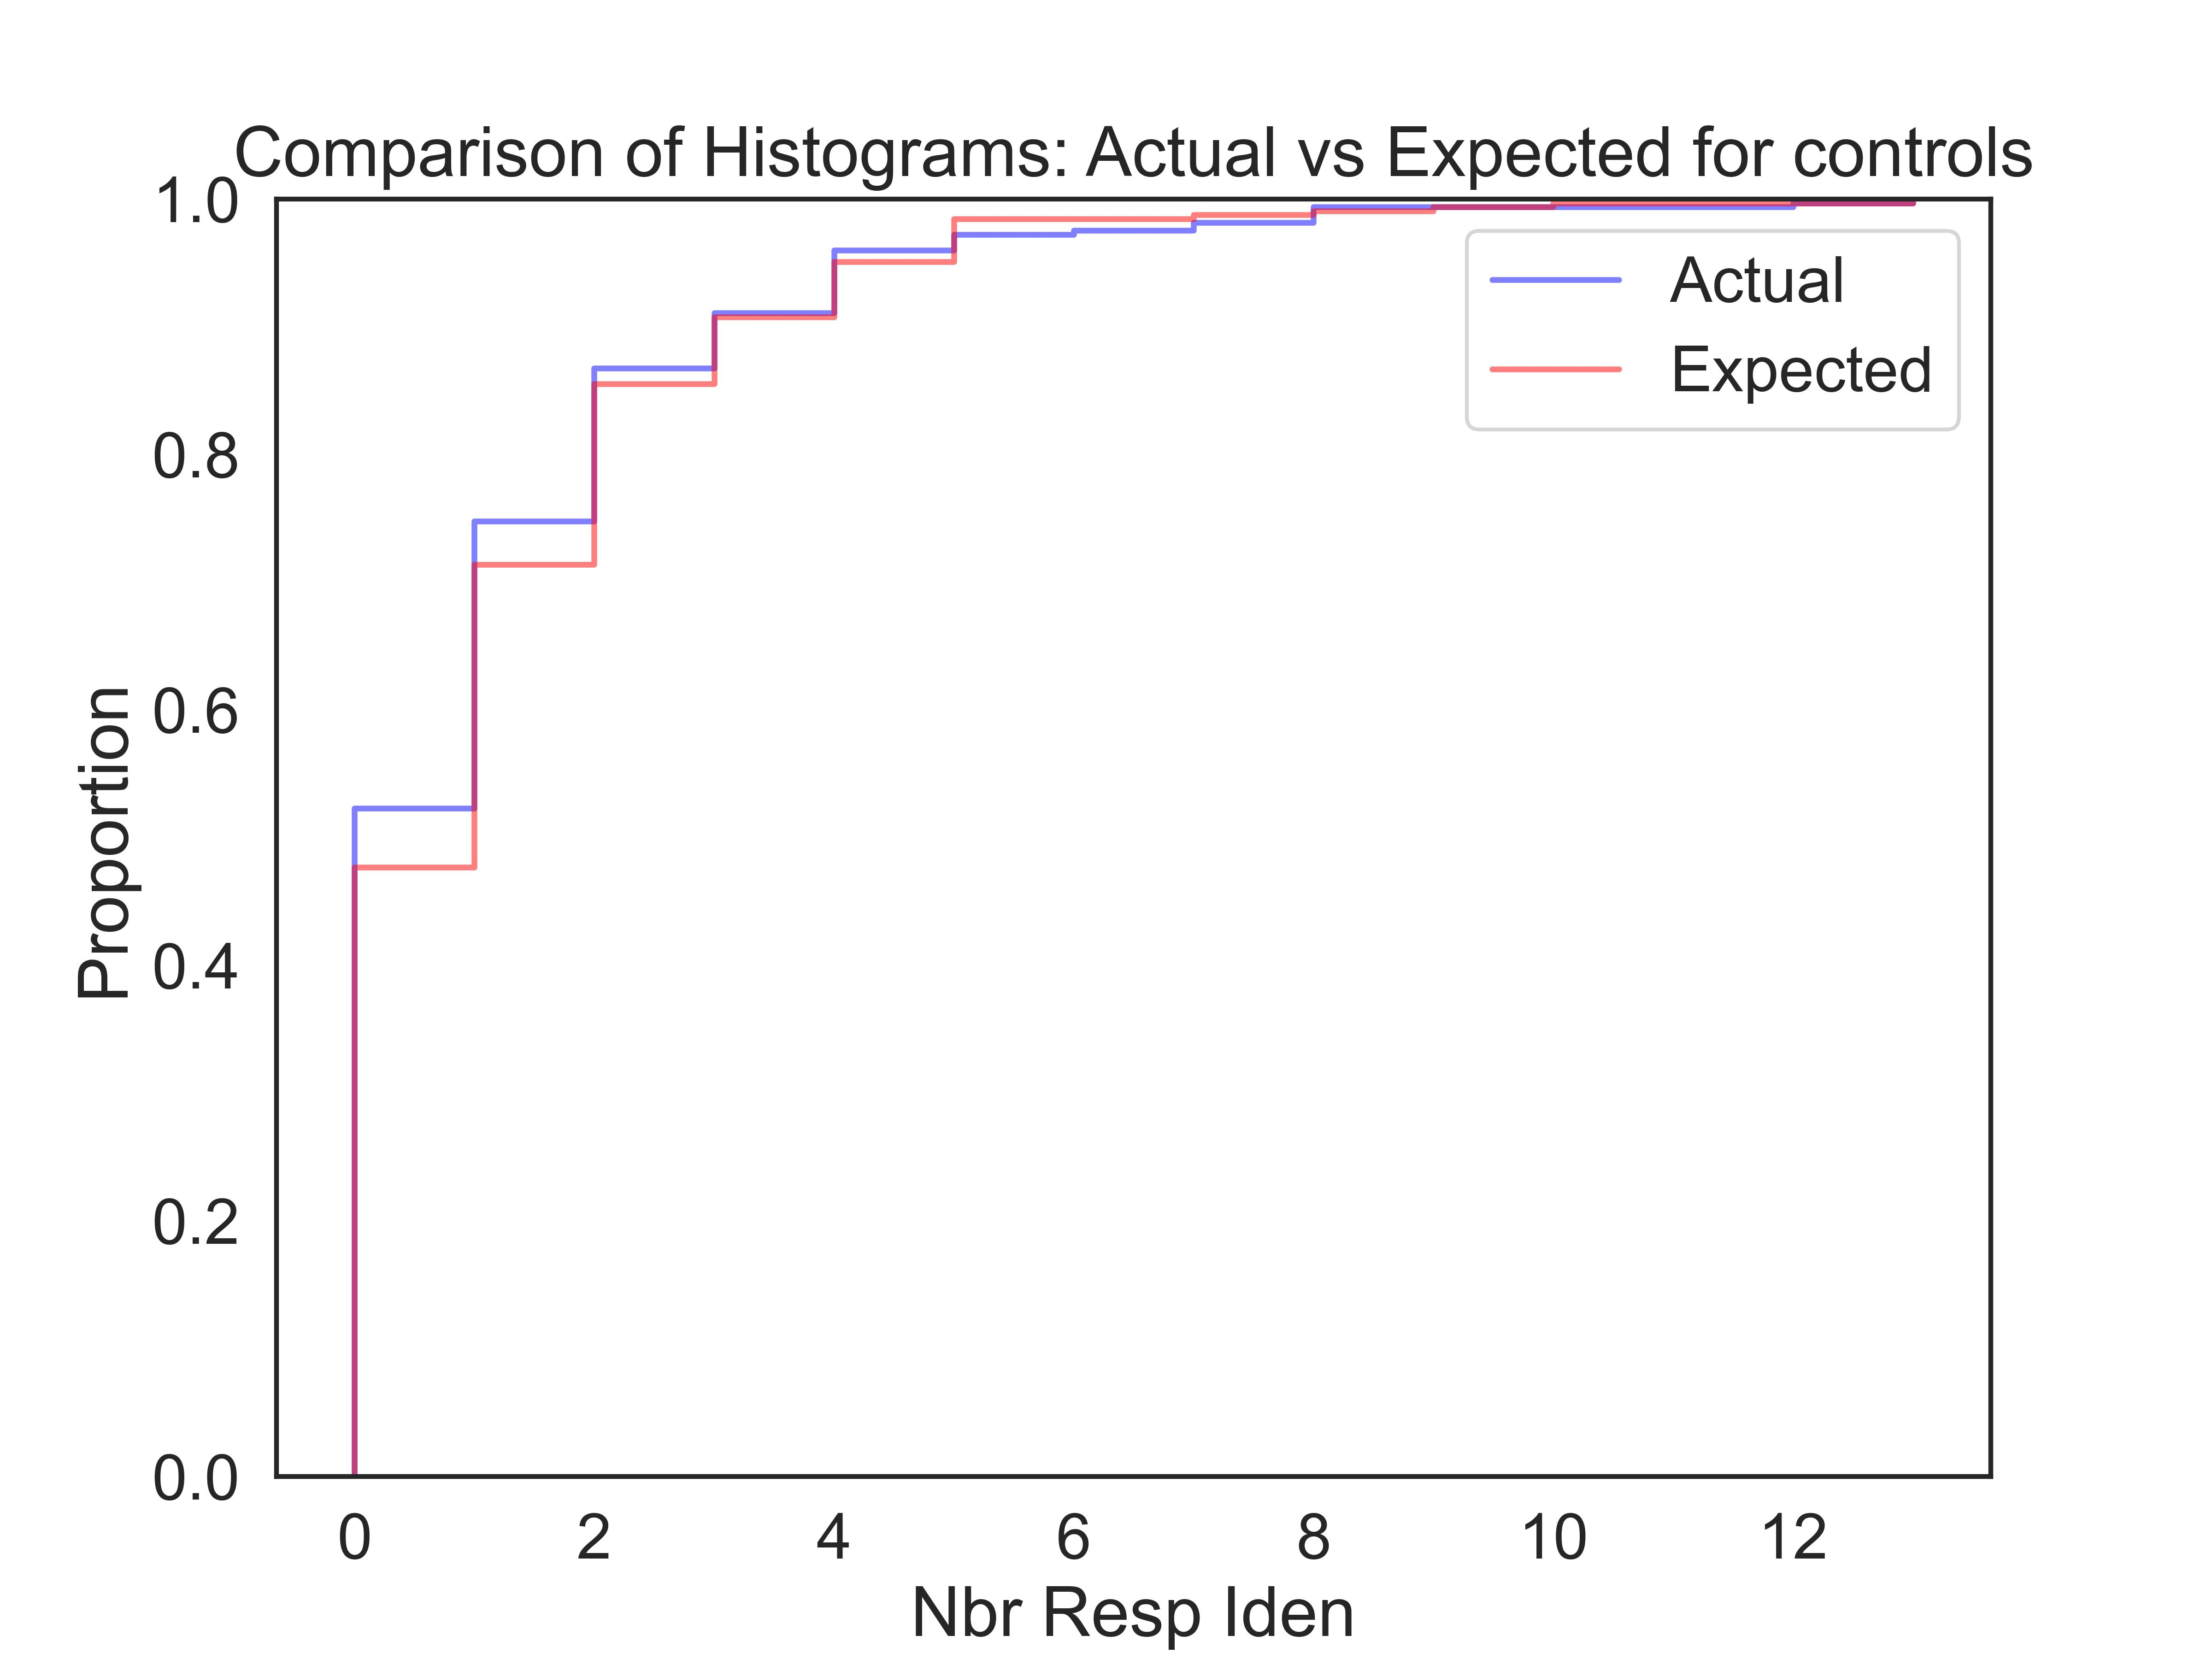
\includegraphics[width=12cm,height=7cm]{MainLayout/Images/chapter9/actual_expected_controls_ecdf.jpg}
    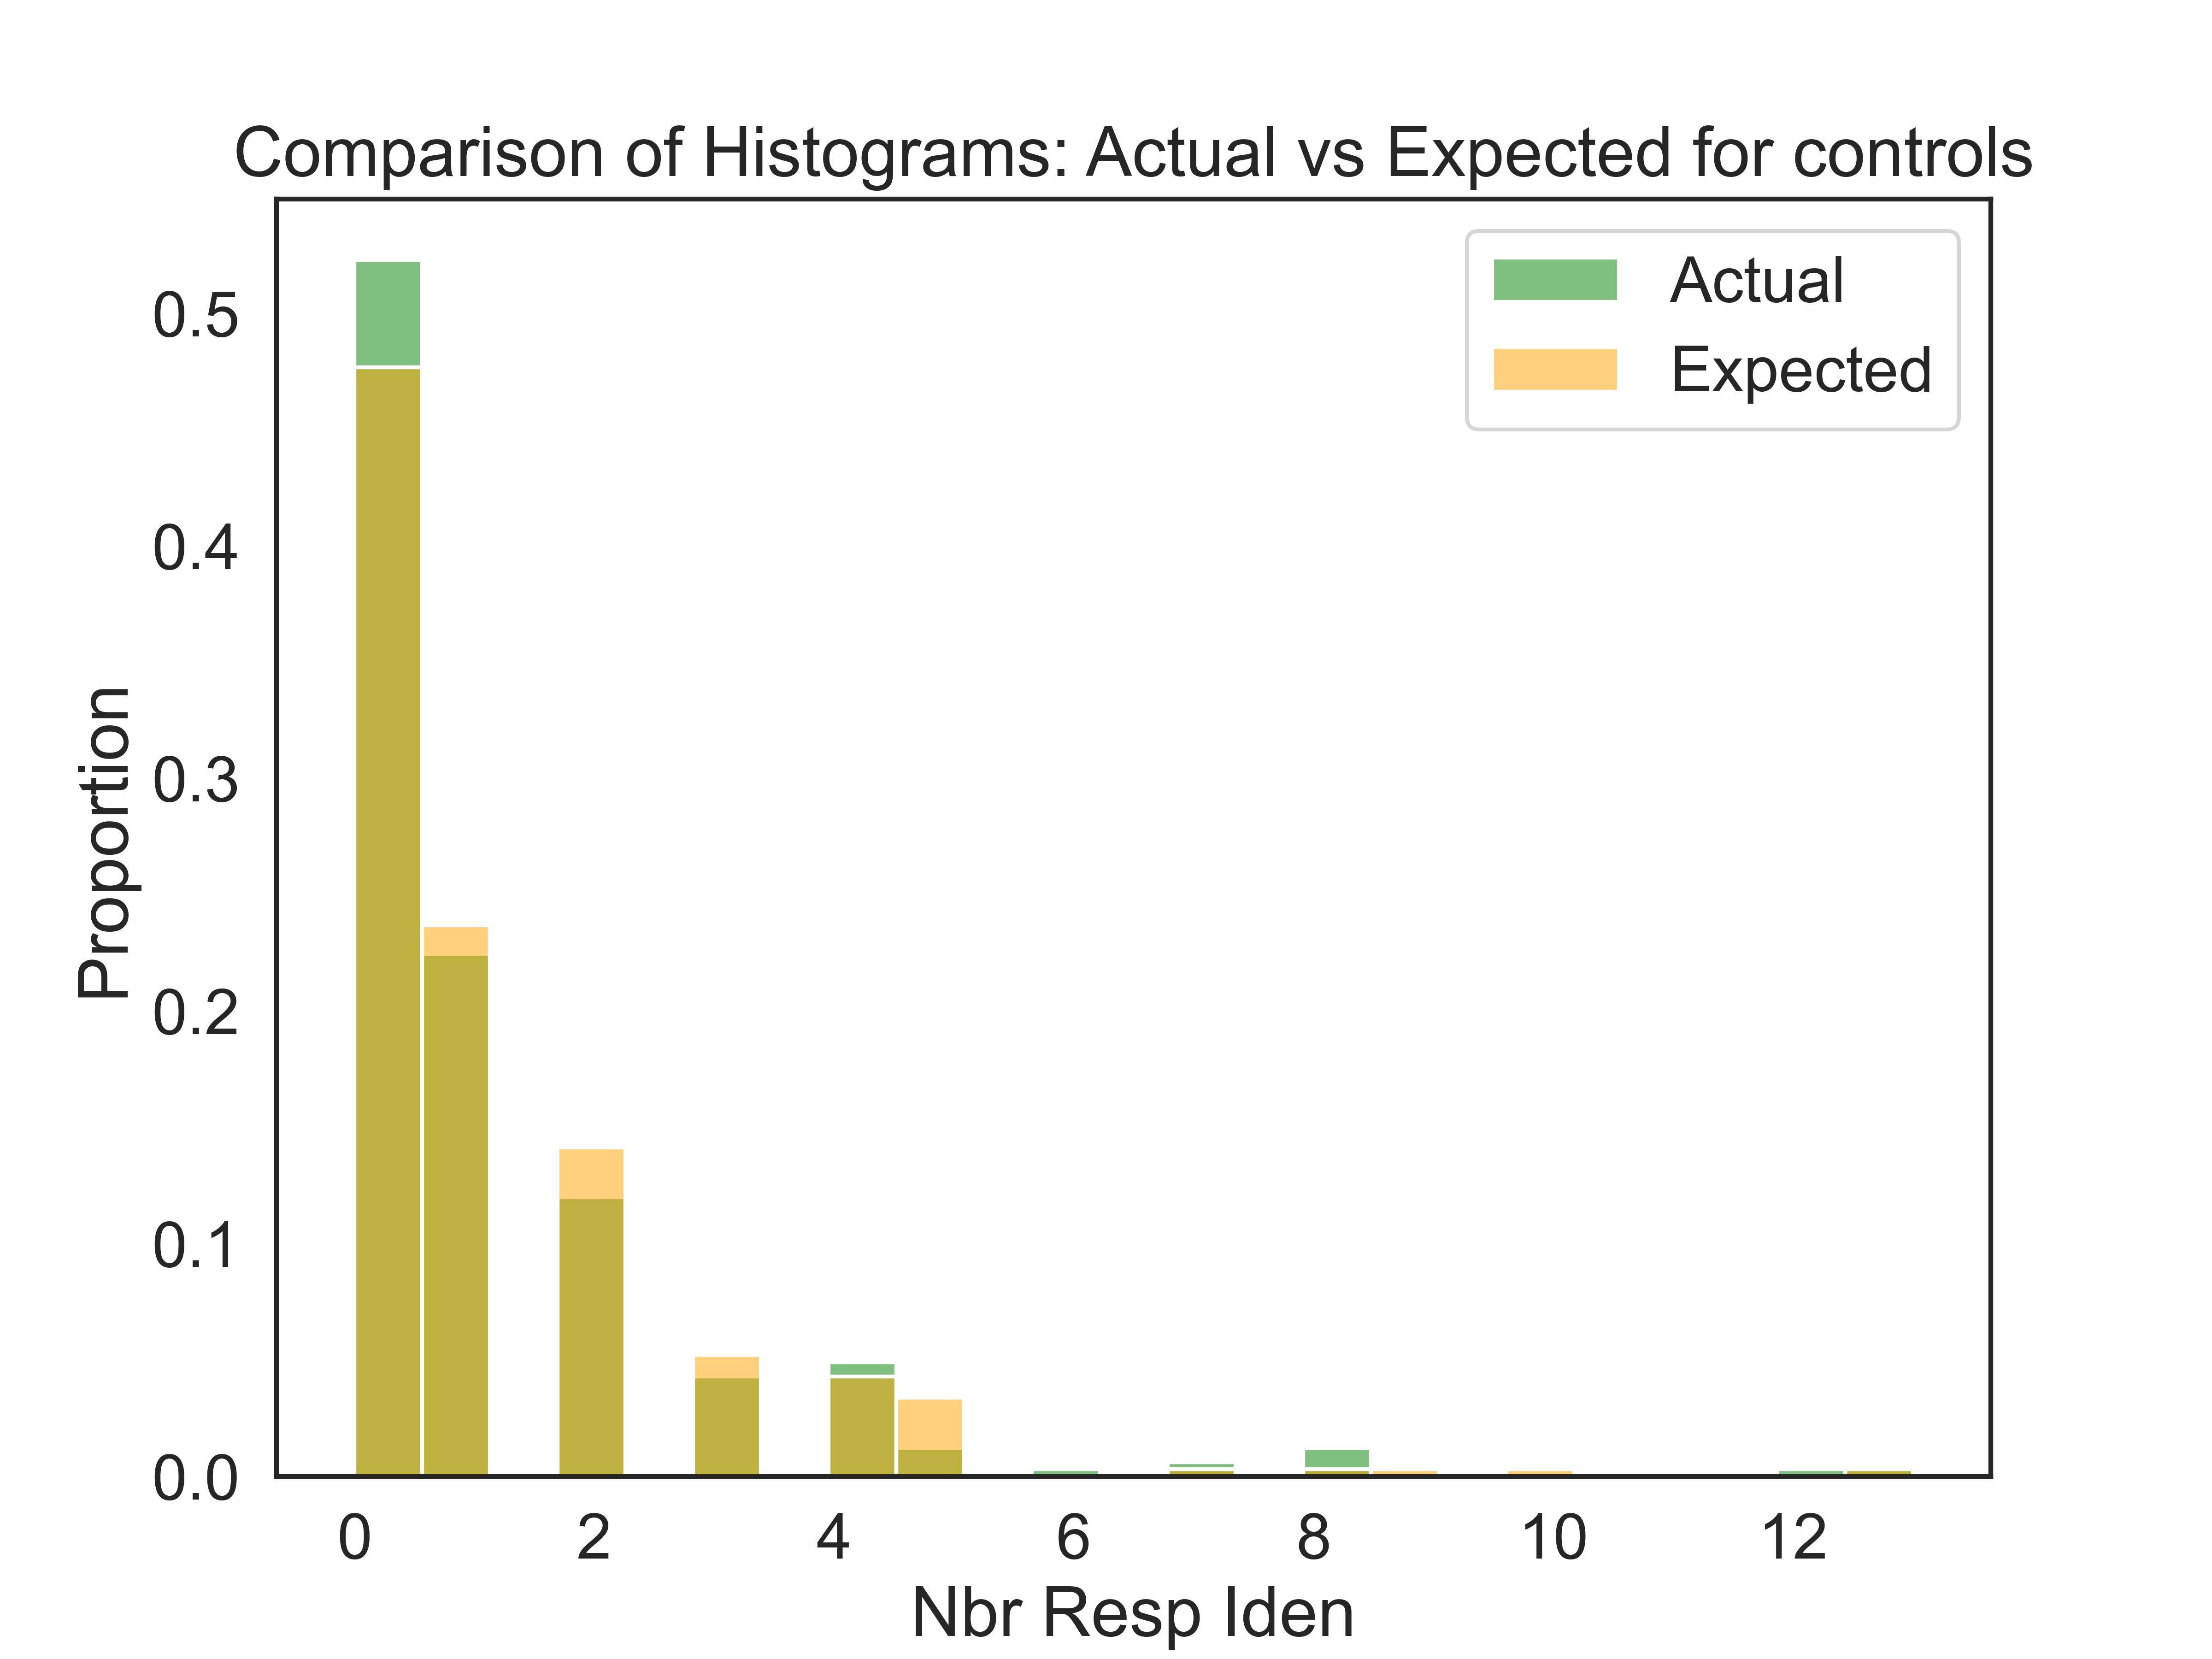
\includegraphics[width=12cm,height=7cm]{MainLayout/Images/chapter9/actual_expected_controls_hist.jpg}
    \caption{Main Title for First Image \\ \small Subtitle for the first graphic.}
    \label{fig:kernel_comparison_methods}
\end{figure}


\begin{figure}[H]
    \centering
    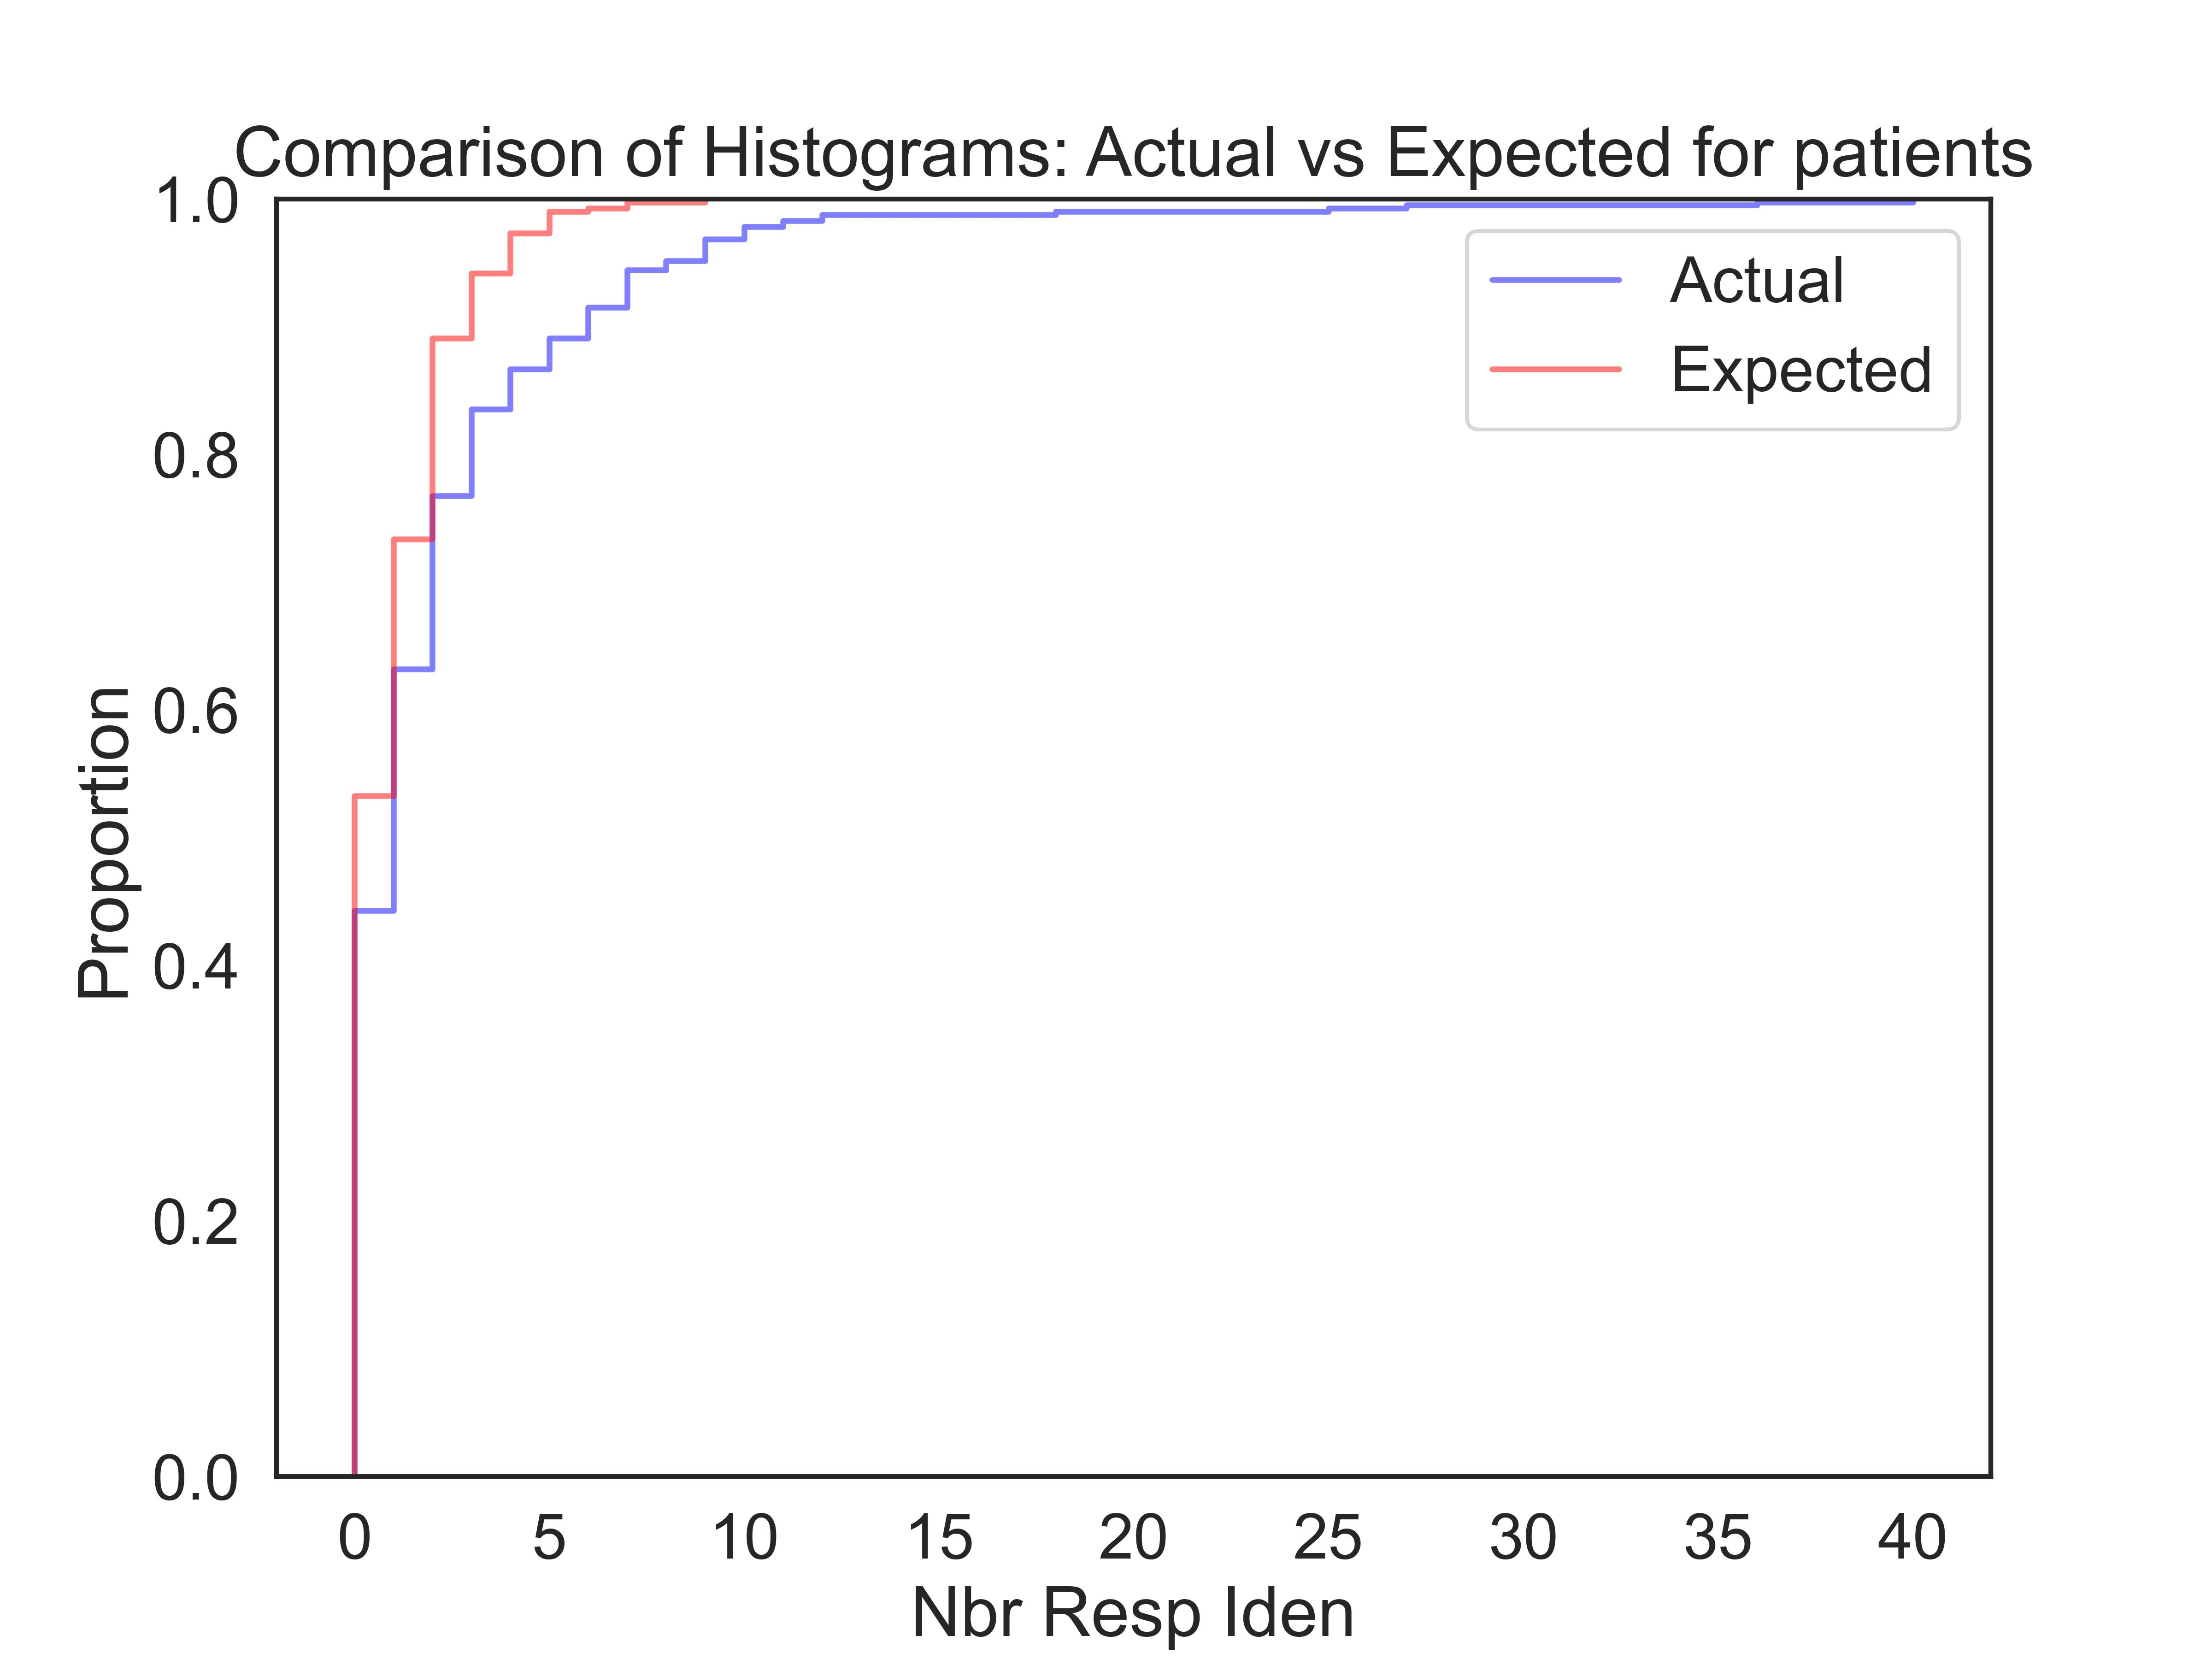
\includegraphics[width=12cm,height=7cm]{MainLayout/Images/chapter9/actual_expected_patients_ecdf.jpg}
    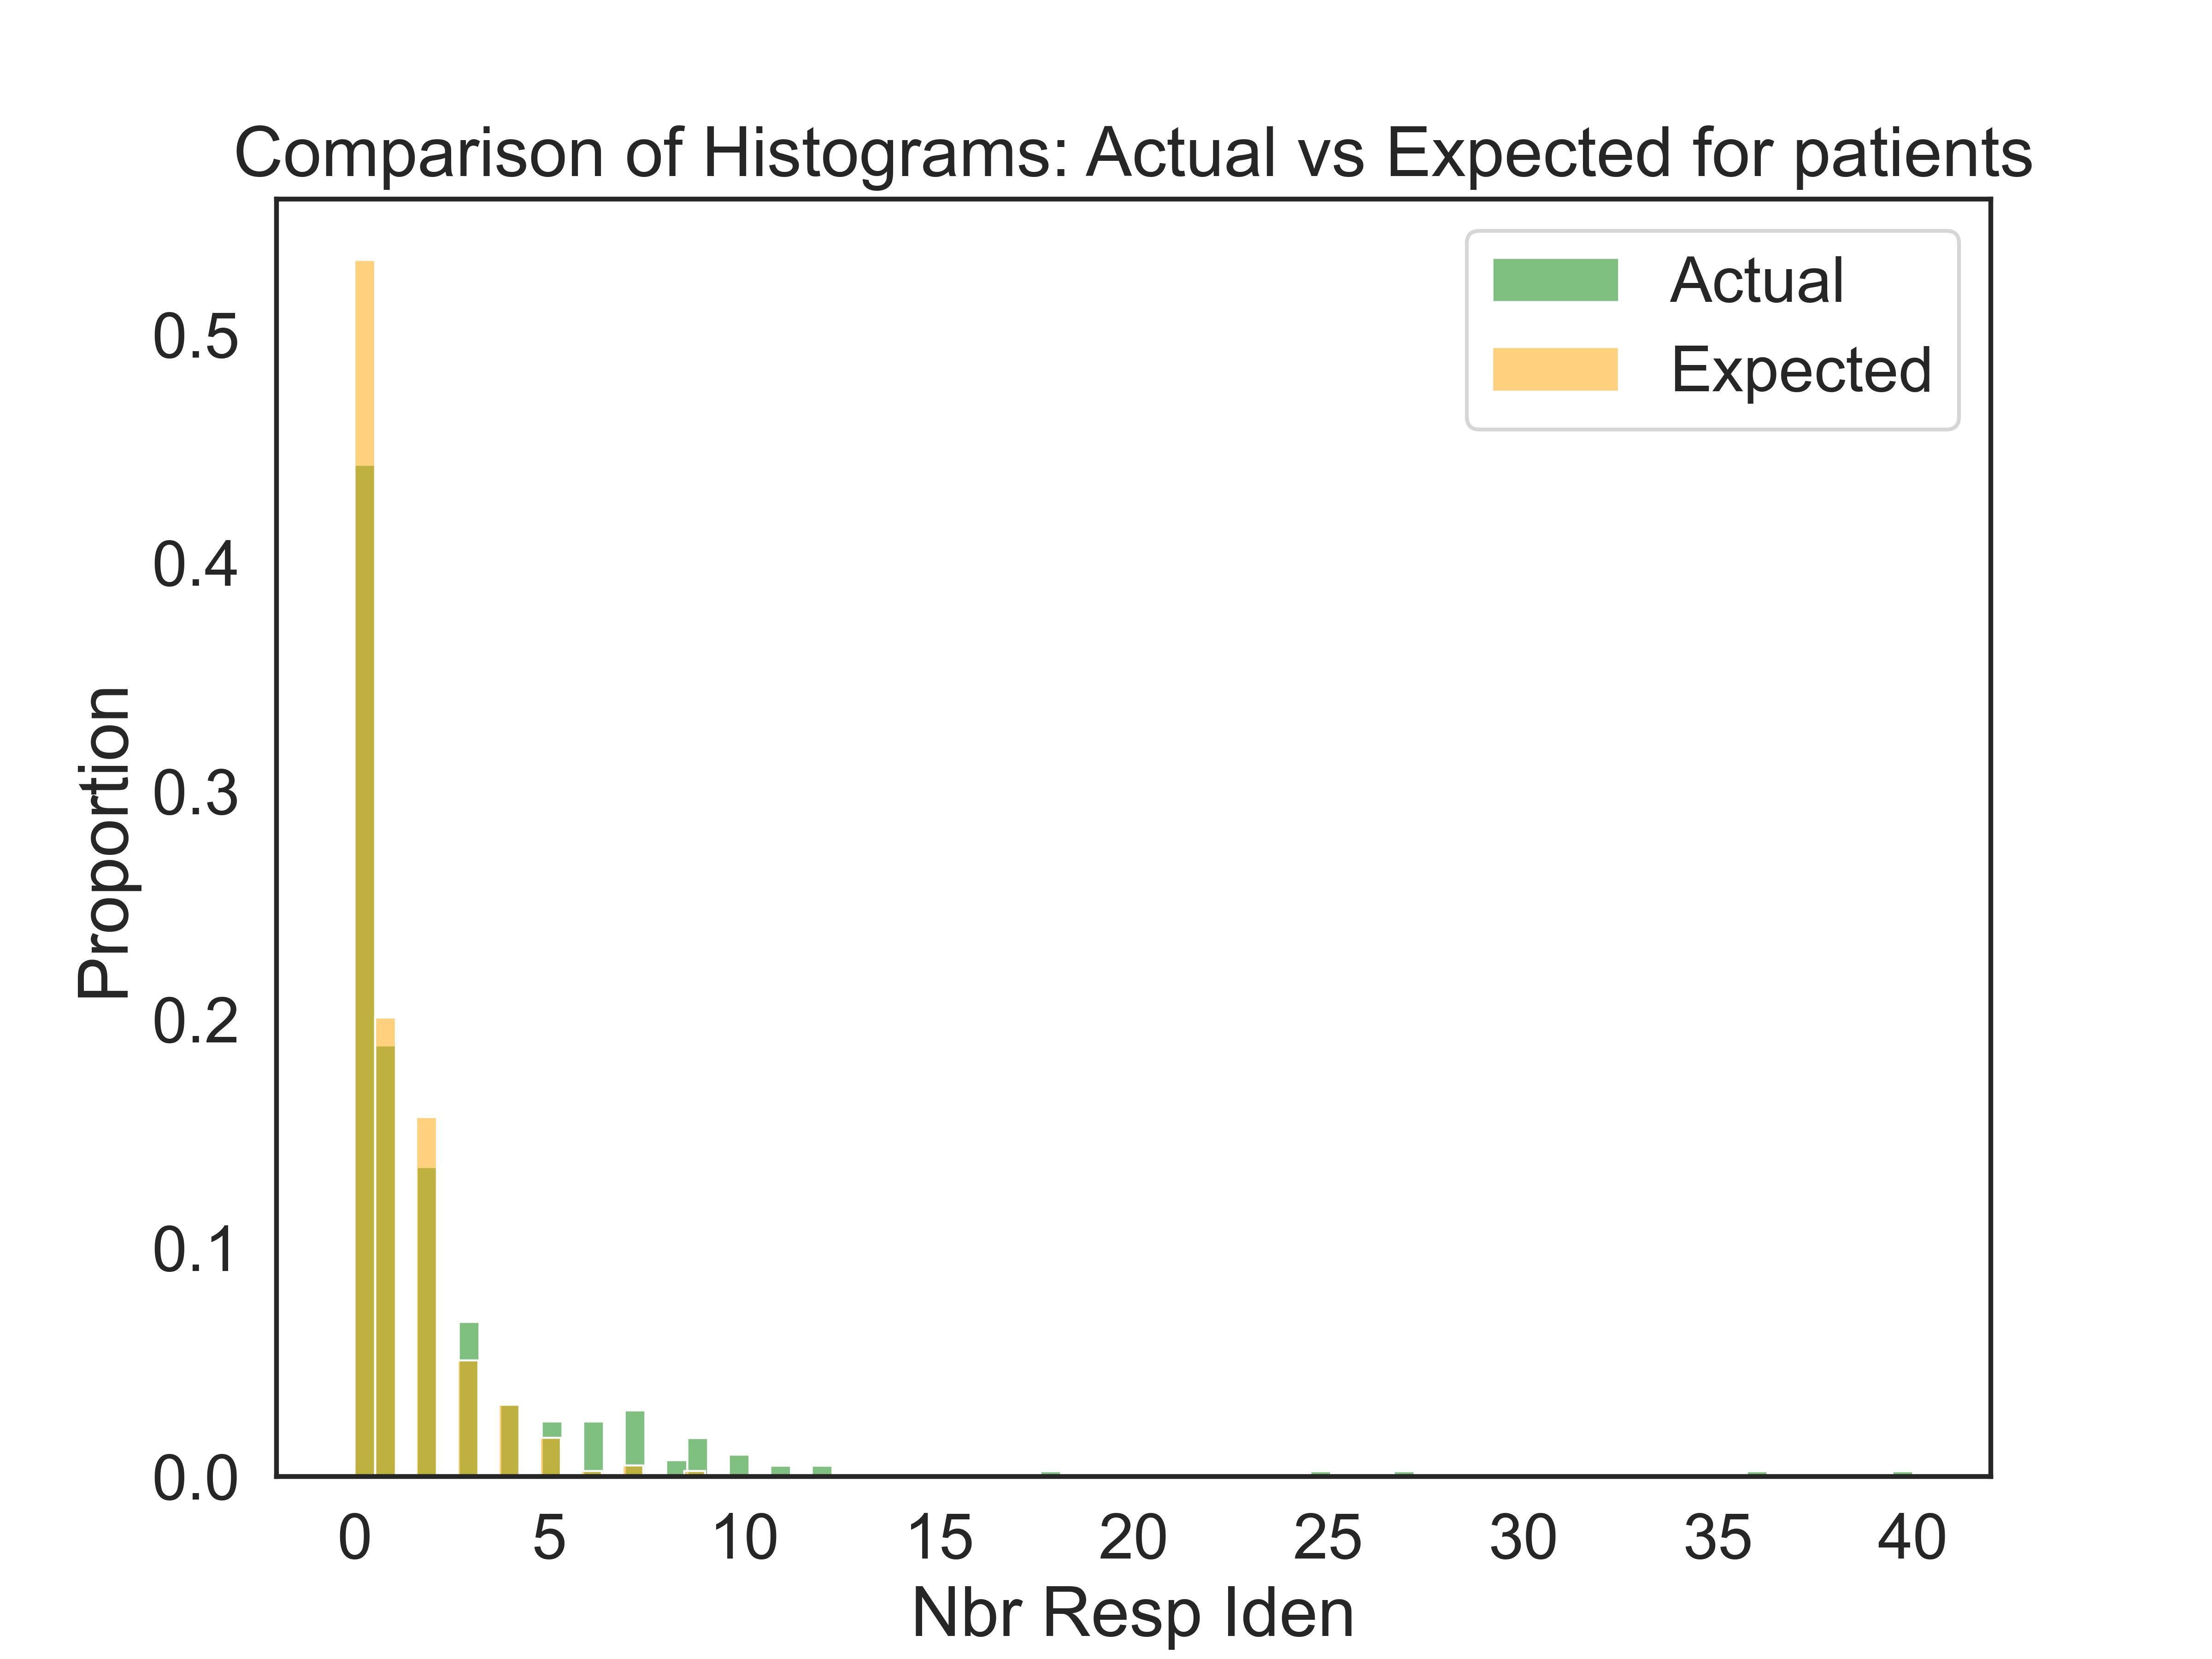
\includegraphics[width=12cm,height=7cm]{MainLayout/Images/chapter9/actual_expected_patients_hist.jpg}
    \caption{Main Title for First Image \\ \small Subtitle for the first graphic.}
    \label{fig:kernel_comparison_methods}
\end{figure}
\subsection{Accuracy} 

\section {Discussion} 

